\documentclass[polish,12pt]{aghthesis}
% \documentclass[english,12pt]{aghthesis} dla pracy w jêzyku angielskim. Uwaga, w przypadku strony tytu³owej zmiana jêzyka dotyczy tylko kolejno¶ci wersji jêzykowych tytu³u pracy. 

% Szablon przystosowany jest do druku dwustronnego. 

\usepackage[T1]{fontenc}
\usepackage[utf8]{inputenc}
\usepackage{url}

\author{Mateusz Bielesz, Wojciech Kosior, Marek Moryl, Kamil Szarek}

\titleProject{Weryfikacja poprawności wyników zwracanych przez serwery DNS \linebreak dla serwisu klienta}

\titleDocument{Opis problemu\\Wizja rozwiązania}

\fieldofstudy{Informatyka}

\supervisor{mgr\ inż.\ Witold Rakoczy}


\date{\the\year}


\begin{document}

\maketitle

\section{Opis problemu}

\subsection{Wstęp}

\hspace{0.5cm} DNS, czyli System Nazw Domenowych (Domain Name System), to system, którego zadaniem jest tłumaczenie nazw domenowych rozumianych przez człowieka na adresy IP, które są przyporządkowane do komputerów i innych urządzeń w sieci internet. Protokół DNS realizowany jest w czterech krokach:

\begin{itemize}
\item wpisujemy adres strony do przeglądarki (np. www.agh.edu.pl),
\item nasze urządzenie wyśle zapytanie do serwera DNS, dotyczące szukanej strony,
\item serwer DNS zwróci IP, pod którym dana strona jest dostępna (np. 149.156.96.52),
\item nasze urządzenie będzie używało zwróconego IP, odwołując się do danej strony internetowej.
\end{itemize}


Proces ten jest bardzo szybki i efektywny, jednak może być skompromitowany poprzez atak hakerski. Możemy mieć do czynienia z przejęciem DNS (DNS hijacking), które spowoduje, że po wysłaniu zapytania o adres konkretnej strony, zostanie nam zwrócone błędne IP, które przekieruje nas na zupełnie inną witrynę. 

\vspace{0.5cm}
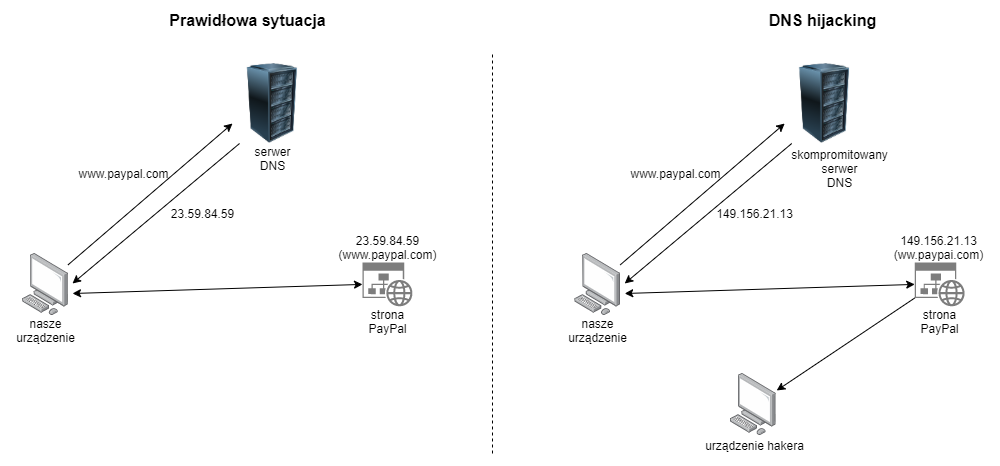
\includegraphics[scale=0.4]{hijackingDNS.png}
\vspace{0.5cm}
 
Taki proceder może być szczególniej niebezpieczny, gdy wymieniane są dane wrażliwe, dotyczące na przykład usług finansowych, w tym naszego konta bankowego czy stron typu PayPal. Podstawiona strona może do złudzenia przypominać wyglądem i funkcjonalnością stronę oryginalną, lecz wszystkie podane przez nas informacje trafią do hakera, który ten atak zainicjował. 

\subsection{Sfałszowanie strony}

\hspace{0.5cm} Warto tutaj zaznaczyć, że obecnie można zobaczyć tendencję do zmiany protokołu przesyłania danych w sieci internet, z nieszyfrowanego HTTP, na o wiele bezpieczniejszy, szyfrowany HTTPS. Dotyczy to także przesyłania plików w sieci - coraz więcej stron używa szyfrowanego protokołu FTPS w miejsce nieszyfrowanego FTP. Ma to związek z presją wywieraną przez fakt, że nieszyfrowane strony coraz częściej są oznaczane przez Google oraz różne przeglądarki internetowe za niebezpieczne. Protokół szyfrujący dane nie tylko zapewnia niemożliwość odczytania danych, które są wymieniane pomiędzy naszym urządzaniem a serwerem na którym działa strona internetowa (man-in-the-middle attack), poprzez zapewnienie szyfrowania asymetrycznego, ale także wymaga autentykacji przy nawiązywaniu połączenia. Wymagany jest certyfikat, wystawiany przez centrum certyfikacji (CA - Certificate Authority), który uzyskać może dowolna osoba lub organizacja, lecz ubieganie się o niego wiąże się z potrzebą potwierdzenia tożsamości i zarejestrowania strony internetowej. Istnieją jednak metody, które mogą pozwolić na ominięcie tego problemu i pozwolą na zadziałanie takiego ataku. Do takich przypadków możemy zaliczyć:

\begin{itemize}
\item  użycie podrobionego certyfikatu, samodzielnie stworzonego, przed którym przeglądarka powinna nas ostrzec, lecz ostrzeżenie to można zignorować i używać podrobionej strony,
\item wykradzenie klucza prywatnego z firmy, która posiada ważny certyfikat, które może być wykonane przez atak z zewnątrz lub pracownika firmy, 
\item wykorzystanie luk w procedurze rejestracyjnej, z której korzysta CA i otrzymanie klucza do strony która nie należy do wnioskodawcy,
\item zhakowanie CA i wygenerowanie potrzebnych kluczy,
\item wymuszenie użycia słabszego algorytmu szyfrującego, w przypadku, gdy użytkownik używa starszej wersji protokołu szyfrującego - SSL 2.0.
\end{itemize}

Oczywiście, nowoczesne przeglądarki w większości tych przypadków powinny wyświetlić komunikat ostrzegający użytkownika, lecz może on ostać zignorowany, lub użytkownik może używać starego, dawno nie aktualizowanego oprogramowania. 

Należy też dodać, że wciąć wiele stron używa protokołów HTTP i FTP, które nie szyfrują danych oraz nie posiadają certyfikatu potwierdzającego oryginalność strony, przez co użytkownicy są narażeni na przejęcie przesyłanych danych, które mogą być łatwo odczytane, lub na podstawienie podobnej strony w miejsce oryginalnej, wykorzystując omawiane przejęcie DNS. 

\subsection{Zmiana wpisu w serwerze DNS}

\hspace{0.5cm} Jak już istnieje strona która łudząco przypomina oryginał, następnym krokiem jest przekierowanie użytkownika tak, aby z niej skorzystał. Z uwagi na ogromny rozmiar internetu i wielość stron które obecnie działają, niemożliwym jest postawienie jednego serwera DNS, który dla każdej strony zwracałby IP, do którego użytkownik powinien się odnieść. Dlatego też zapytanie użytkownika przechodzi przez kilka takich serwerów, z których każdy odpowiada za bardziej złożony adres. Tutaj pojawia się ryzyko, ponieważ wystarczy  aby jeden z nich zwrócił niepoprawne dane i zapytanie może się nie udać, lub co gorsza, użytkownikowi może zostać zwrócone IP niezgodne z tym, które przynależy do szukanej strony. Taki proceder może zaistnieć w przypadku:

\begin{itemize}
\item skompromitowania prawdziwego serwera DNS przez hakera, który, jeśli dostanie dostęp, może dowolnie zmieniać i edytować zawarte tam reguły, przekierowując wybrane zapytania na inny, kontrolowany przez siebie serwer,
\item celowej zmiany wyników zwracanych przez serwer DNS, spowodowanej naciskami akcjonariuszy lub rządu, na którego terenie dany serwer DNS działa.
\end{itemize}

Na świecie istnieje wiele serwerów DNS, które dzielą ruch pomiędzy siebie. W wyniku skompromitowania jednego z niech może wystąpić sytuacja, że użytkownik strony z obszaru obsługiwanego przez dany, skompromitowany serwer zostanie przekierowany na kontrolowaną przez hakera kopię strony, a w pozostałych regionach świata użytkownicy będą kierowani do oryginału. 

Jedną możliwością uchronienia się przed takim atakiem jest odpytywanie serwerów DNS w różnych zakątkach świata i sprawdzanie, czy zwracana zawartość jest tożsama z oczekiwaną. Użytkownik może wykonać takie zadanie ręcznie, przy użyciu przeglądarki i VPNa, lecz w naszym projekcie chcielibyśmy ten proces zautomatyzować i zapewnić serwis, który dla wielu użytkowników i ich stron internetowych mógłby cyklicznie odpytywać serwery DNS na świecie i sprawdzać, czy zwracane dane zgadzają się z oczekiwanymi.


\newpage

\section{Wizja rozwiązania}

\subsection{Wstęp}

\hspace{0.5cm} Celem produktu, który chcemy dostarczyć, jest zautomatyzowanie zapytań do różnych serwerów DNS, weryfikacja ich poprawności, oraz w razie wykrycia błędnie zwracanego IP, jak najszybsze powiadomienie użytkownika. Aplikacja ma także działać dla wielu użytkowników jednocześnie. Domyślnie użytkownikiem mogłaby stać się dowolna osoba, która posiada własny serwis internetowy i po wykupieniu subskrypcji byłaby chroniona. 

\subsection{Back-end}

\hspace{0.5cm} Pierwszą część naszego projektu stanowiłby program działający na serwerze, który miałby odpytywać cyklicznie serwery DNS na całym świecie o podane przez klientów strony internetowe. W przypadku stwierdzenia nieprawidłowości byłby on w stanie natychmiast poinformować klienta gdzie wystąpił problem tak, aby ten zdołał jak najszybciej zareagować. Mógłby on współpracować z dowolnym VPNem, podanym przez administratora.

\subsection{Front-end}

\hspace{0.5cm} Dla użytkowników udostępniona zostałaby strona internetowa, która umożliwiałaby im interakcję z nasza aplikacją. Nowi użytkownicy musieliby się najpierw zarejestrować, po czym mieliby możliwość wykupienie subskrypcji. Subskrypcja dotyczyłaby jednego lub kilku serwisów, które byłyby regularnie sprawdzane.

Po ponownym zalogowaniu byłaby dla nich dostępna możliwość zarządzania subskrypcjami, wykupienia dodatkowych, oraz sprawdzenia statystyk. Statystyki dotyczyłyby testów wykonanych dla podanych przez nich serwisów.

Na tej samej stronie mógłby się także zalogować administrator systemu, który miałby dostęp do ustawień oraz listy klientów i wykupionych przez nich subskrypcji.

\end{document}
